\section{Results}
\label{sec:results}

Throughout, ``deep noise'' denotes the pre-specified adjudication band $\{0, -2, -6\,\mathrm{dB}\}$; $-10\,\mathrm{dB}$ is reported but excluded from adjudication (the time-invariant baseline is near chance there: a constant majority-class predictor scores $40.0\%$ and a uniformly random predictor $48.6\%$ macro-F1 on this evaluation set, against $52.3\%$ for S4D). All values are macro-F1 (\%), mean over 5 seeds, best-epoch on the evaluation condition (Section~\ref{sec:protocol:report}) unless stated otherwise. Figure~\ref{fig:chain} summarises the three-step ablation chain that structures this section.

\begin{figure}[htbp]
\centering
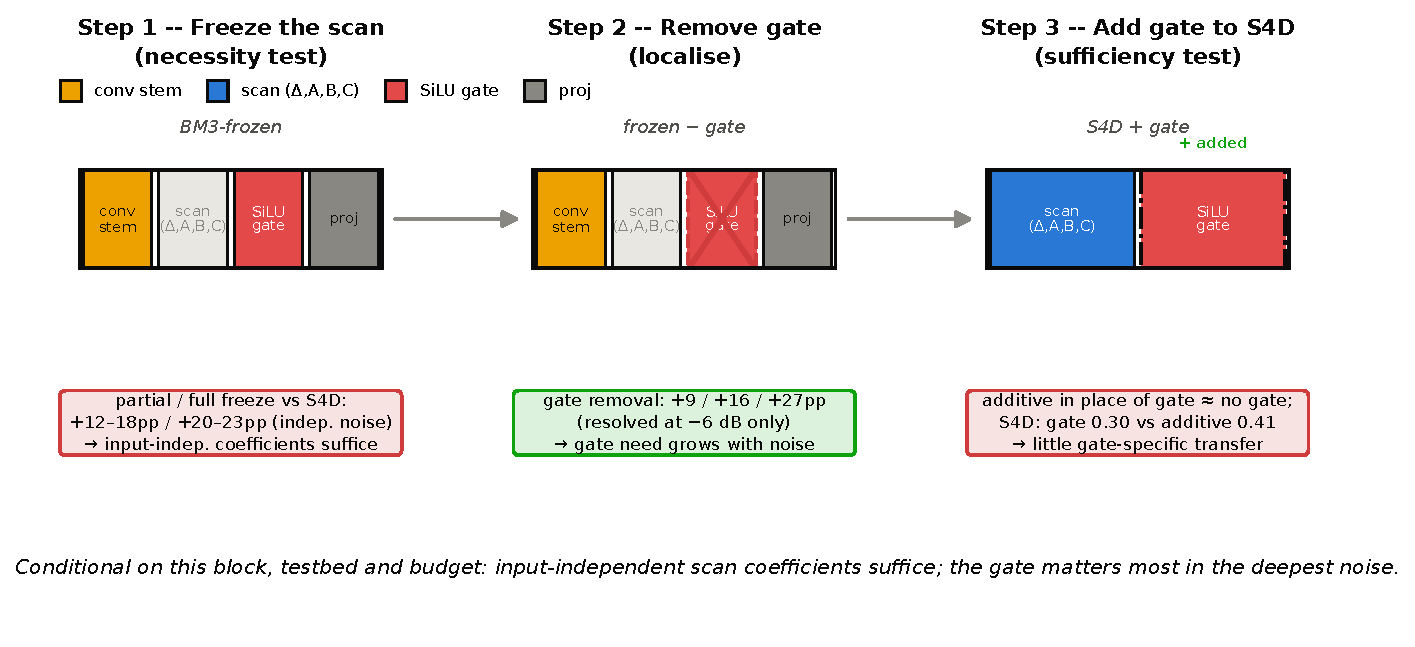
\includegraphics[width=0.85\linewidth]{figures/fig1_chain}
\caption{The three-step ablation chain with pre-specified thresholds: freeze the input-dependent $\Delta,A,B,C$ projections (Section~\ref{sec:results:falsify}), remove one component at a time on the frozen base to localise the necessary ingredient (Section~\ref{sec:results:localise}), and graft that ingredient onto S4D to test sufficiency (Section~\ref{sec:results:graft}).}
\label{fig:chain}
\end{figure}

\subsection{Freezing the input-dependent $\Delta$, $A$, $B$, $C$ projections}
\label{sec:results:falsify}

\begin{table}[htbp]
\centering
\caption{BM3 vs.\ BM3-frozen vs.\ S4D, macro-F1 (\%) by SNR (frozen-selectivity grid). $\Delta$(BM3$-$frozen) and $\Delta$(frozen$-$S4D) in percentage points.}
\label{tab:falsify}
\begin{tabular}{@{}lrrrrr@{}}
\toprule
Condition & BM3 & BM3-frozen & S4D & $\Delta$(BM3$-$frozen) & $\Delta$(frozen$-$S4D) \\
\midrule
clean & 78.9 & 78.9 & 81.0 & $-0.0$ & $-2.1$ \\
0\,dB & 95.0 & 89.9 & 76.1 & $+5.1$ & $\mathbf{+13.8}$ \\
$-2$\,dB & 95.4 & 92.1 & 75.1 & $+3.3$ & $\mathbf{+17.0}$ \\
$-6$\,dB & 88.5 & 86.3 & 68.5 & $+2.2$ & $\mathbf{+17.7}$ \\
$-10$\,dB\rlap{$^{*}$} & 68.1 & 64.3 & 52.3 & $+3.8$ & $+12.0$ \\
\bottomrule
\end{tabular}
\end{table}

\begin{figure}[htbp]
\centering
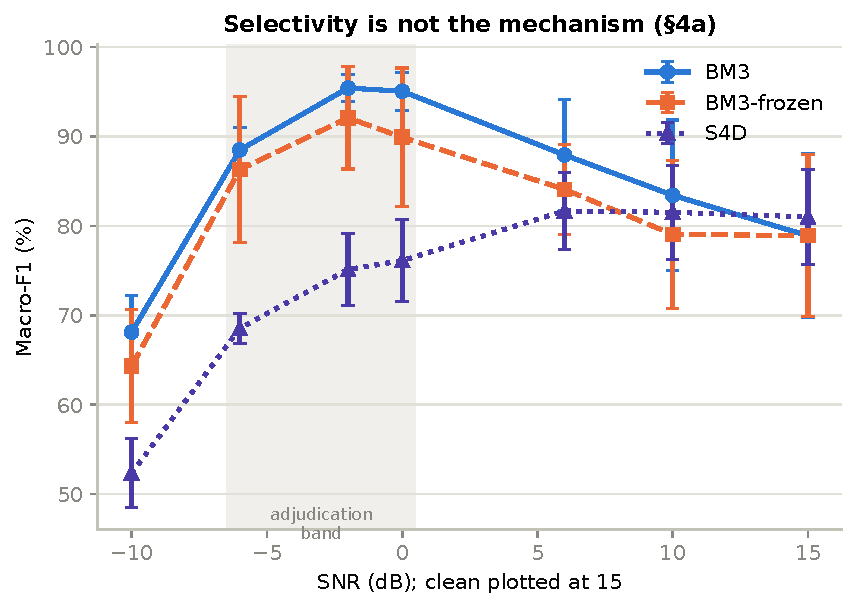
\includegraphics[width=0.85\linewidth]{figures/fig2_snr_curves}
\caption{Macro-F1 vs.\ SNR for BM3, BM3-frozen, and S4D across the full noise grid. The frozen arm tracks BM3 closely and stays well above S4D throughout the adjudication band.}
\label{fig:snr_curves}
\end{figure}

Freezing the input-dependent $\Delta$, $A$, $B$, $C$ projections (Section~\ref{sec:protocol:freeze}) costs at most $5.1\pp$ anywhere in the adjudication band on the point estimates, while the frozen block retains a $13.8$--$17.7\pp$ advantage over S4D (Table~\ref{tab:falsify}, Figure~\ref{fig:snr_curves}). Five seeds bound these quantities loosely: paired 95\% intervals for $\Delta$(BM3$-$frozen) are $[-4.7, 15.0]$, $[-3.1, 9.8]$ and $[-7.5, 11.8]\pp$ at $0$, $-2$ and $-6$\,dB (BM3 ahead in 3/5, 4/5 and 2/5 seeds), and for $\Delta$(frozen$-$S4D) $[-0.5, 28.0]$, $[5.5, 28.4]$ and $[5.8, 29.7]\pp$ (5/5, 5/5, 5/5 seeds). The pre-specified rule attributed robustness to selectivity only if $\Delta$(BM3$-$frozen) $\geq 10\pp$ in deep noise with the frozen arm collapsing toward S4D. Neither condition holds on the point estimates, so the pre-specified verdict is that these projections are \emph{not the primary mechanism}. This is a failure to meet a confirmation criterion, not a demonstration that freezing is cheap: the intervals above are compatible with differences larger than $10\pp$, and no equivalence margin was pre-specified or tested. One limit applies: the frozen arm still contains input-dependent trapezoidal weights and rotation angles, so this result concerns $\Delta, A, B, C$ only; Section~\ref{sec:results:fullfreeze} removes that limit. Under last-epoch reporting the re-run gives $\Delta$(BM3$-$frozen) $= +3.7$, $+0.9$ and $+0.2\pp$ (best-epoch re-run: $+5.1$, $+3.5$, $+3.0\pp$; intervals still include zero at every level), so the point estimates fall further below the $10\pp$ threshold rather than rising towards it. On clean data S4D matches or slightly exceeds both Mamba-style arms---consistent with the systematic clean-TSC comparison~\cite{saadatmand2026s4d}. In the noisy regime, the block's advantage over S4D is not removed by freezing these four terms, so it must be carried by other parts of the block or by the remaining input-dependent scan terms.

\subsection{Freezing the remaining input-dependent scan terms}
\label{sec:results:fullfreeze}

Table~\ref{tab:fullfreeze} reports the three layered arms of Section~\ref{sec:protocol:freeze} on the adjudication band (60 cells: 4 arms $\times$ 3 levels $\times$ 5 seeds $\times$ 50 epochs, the original training code, the same evaluation fingerprint, with the original BM3 arm re-run in the same grid). The question is whether the advantage that survived freezing $\Delta, A, B, C$ is carried by the two input-dependent terms the frozen arm retained.

\begin{table}[htbp]
\centering
\caption{Layered freezing of the scan's input-dependent terms. Macro-F1 (\%), mean over 5 seeds, under best-epoch and final-epoch reporting; $\Delta$ columns are paired differences under final-epoch reporting with 95\% $t$-intervals over seeds.}
\label{tab:fullfreeze}
\footnotesize\setlength{\tabcolsep}{4pt}
\begin{tabular}{@{}lrrrrrr@{}}
\toprule
 & \multicolumn{2}{c}{0\,dB} & \multicolumn{2}{c}{$-2$\,dB} & \multicolumn{2}{c}{$-6$\,dB} \\
\cmidrule(lr){2-3}\cmidrule(lr){4-5}\cmidrule(lr){6-7}
Arm & best & final & best & final & best & final \\
\midrule
BM3 (re-run) & 95.6 & 86.9 & 95.8 & 88.3 & 88.6 & 83.3 \\
BM3-frozen ($\Delta,A,B,C$) & 90.6 & 83.1 & 92.3 & 87.3 & 85.7 & 83.1 \\
frozen$-$trap & 95.5 & 87.6 & 95.3 & 89.3 & 90.5 & 88.0 \\
frozen$-$rot & 94.6 & 86.7 & 94.6 & 89.1 & 89.0 & 86.4 \\
frozen$-$all & 96.5 & 89.5 & 96.8 & 91.5 & 90.5 & 87.9 \\
S4D & 75.9 & 67.6 & 75.1 & 67.5 & 68.6 & 66.7 \\
\midrule
\multicolumn{7}{@{}l}{\emph{Paired differences, final-epoch reporting (pp)}} \\
frozen$-$all $-$ S4D & \multicolumn{2}{c}{$+21.9$ [16.7, 27.1]} & \multicolumn{2}{c}{$+24.0$ [21.4, 26.5]} & \multicolumn{2}{c}{$+21.2$ [17.5, 24.9]} \\
BM3-frozen $-$ frozen$-$all & \multicolumn{2}{c}{$-6.3$ [$-$17.6, 4.9]} & \multicolumn{2}{c}{$-4.1$ [$-$12.0, 3.7]} & \multicolumn{2}{c}{$-4.8$ [$-$17.8, 8.2]} \\
BM3 $-$ frozen$-$all & \multicolumn{2}{c}{$-2.6$ [$-$8.2, 2.9]} & \multicolumn{2}{c}{$-3.2$ [$-$7.0, 0.6]} & \multicolumn{2}{c}{$-4.5$ [$-$7.2, $-$1.9]} \\
\bottomrule
\end{tabular}
\end{table}

It is not. With every tensor entering the scan input-independent, \emph{frozen$-$all} is $+21.9$, $+24.0$ and $+21.2\pp$ above S4D at $0$, $-2$ and $-6$\,dB under final-epoch reporting, positive in 5/5 seeds at every level and with intervals excluding zero---if anything a larger margin than the partially frozen arm's $+15.5$, $+19.8$, $+16.4\pp$ (Table~\ref{tab:sensitivity_contrasts}). None of the three freezing steps costs accuracy: the paired differences BM3-frozen $-$ frozen$-$trap, $-$ frozen$-$rot and $-$ frozen$-$all are negative at all three levels (between $-1.8$ and $-6.3\pp$ under final-epoch reporting), i.e.\ the more heavily frozen arm is numerically ahead, with every interval including zero. The direction is not an artefact of capacity: \emph{frozen$-$all} has 103{,}842 parameters against 112{,}410 for BM3-frozen and 177{,}938 for BM3. At the deepest level \emph{frozen$-$all} also exceeds the full BM3 block by $4.5\pp$ ($[-7.2, -1.9]$ for BM3 $-$ frozen$-$all, 0/5 seeds in BM3's favour); we report this but do not build on it, since five seeds and one speed pair cannot separate a genuine advantage of a time-invariant scan from a variance effect.

Two readings of the whole step are therefore available, and the data do not separate them: input-dependence of the scan contributes nothing measurable here, or it contributes something that the learned constants recover under this training budget. Either way the conclusion for the attribution chain is the same and now rests on a complete intervention rather than a partial one: \textbf{the Mamba-style block's deep-noise advantage over a time-invariant S4D does not require any input-dependent term in its scan}. What remains to carry it is the rest of the block---the convolutional stem, the heavy-tailed $A$ parameterisation, the normalisations and the output gate---which is what Sections~\ref{sec:results:localise}--\ref{sec:results:graft} examine. The re-run also reproduces the original grids: the BM3 arm's best-epoch means (95.6, 95.8, 88.6) exceed Table~\ref{tab:falsify}'s 95.0, 95.4, 88.5 by $0.57$, $0.43$ and $0.16\pp$ (a different PyTorch/Triton build, Section~\ref{sec:results:sensitivity}).

\subsection{Removing the gate is the only ablation with a large, one-signed effect}
\label{sec:results:localise}

\begin{table}[htbp]
\centering
\caption{Single-component removal on the frozen base (component-ablation grid, trained separately from Table~\ref{tab:falsify}), $\Delta$(frozen $-$ arm) in percentage points.}
\label{tab:localise}
\begin{tabular}{@{}lrrrp{4.0cm}@{}}
\toprule
Component removed & 0\,dB & $-2$\,dB & $-6$\,dB & Adjudication \\
\midrule
SiLU gate & $\mathbf{+13.1}$ & $\mathbf{+21.1}$ & $\mathbf{+23.5}$ & PRIMARY (all $\geq 8\pp$) \\
conv stem ($k{=}7$) & $-6.6$ & $-2.7$ & $+7.9$ & outside pre-specified bins (regime trade-off) \\
heavy-tailed $A \rightarrow$ S4D-style $A$ & $-2.4$ & $-2.2$ & $-4.2$ & outside bins (removal numerically beneficial; intervals include 0) \\
\bottomrule
\end{tabular}
\end{table}

\begin{figure}[htbp]
\centering
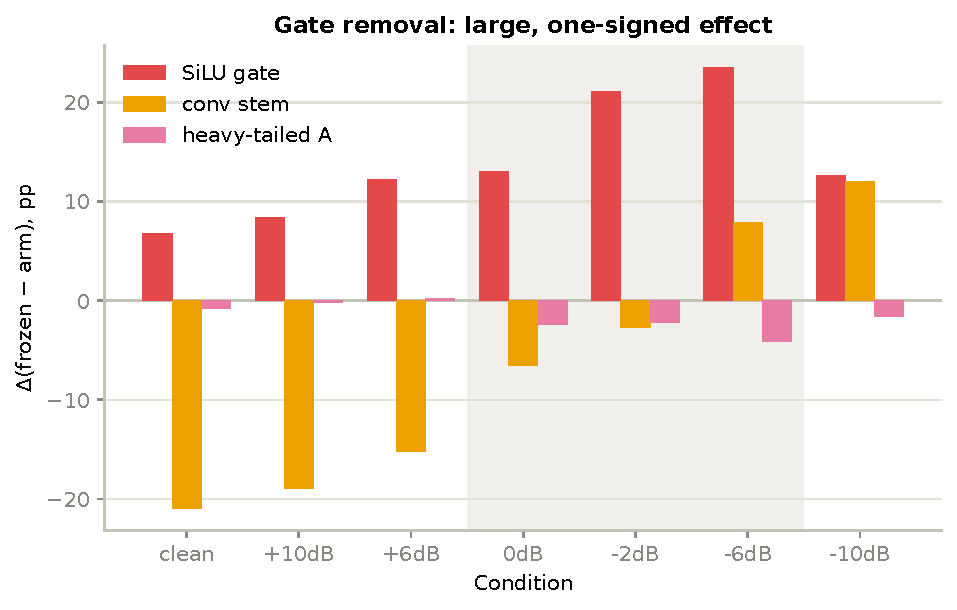
\includegraphics[width=0.85\linewidth]{figures/fig3_ablation_bars}
\caption{Component-removal $\Delta$ (percentage points, frozen $-$ arm) by SNR for the three single-component ablations on the frozen base. Only gate removal is monotone, large, and one-signed across the adjudication band.}
\label{fig:ablation_bars}
\end{figure}

``Necessary'' is used here in the operational sense of this ablation: removing the gate from the frozen block, with the other components and the budget unchanged, removes most of the block's advantage. The gate result is large, one-signed and monotone in noise depth: removal costs $13.1$, $21.1$ and $23.5\pp$ at $0$, $-2$ and $-6$\,dB (paired 95\% intervals $[6.5, 19.6]$, $[3.8, 38.5]$, $[8.5, 38.6]\pp$; 5/5 seeds at every level). The gateless arm also gives up most of the Mamba advantage: it sits \textbf{below plain S4D} at $-2$\,dB (71.7 vs.\ 75.2) and $-6$\,dB (62.5 vs.\ 68.6), though not at $0$\,dB (77.6 vs.\ 76.2), and the gateless--S4D gap itself is not resolved by five seeds (Section~\ref{sec:results:sensitivity}: under last-epoch reporting the gateless arm is below S4D at $-6$\,dB only). We read this as ``at best on par with S4D, and worse at the deepest noise level'', which suggests, but does not establish, that components interact rather than add. The other two components tell regime stories rather than robustness stories: the convolutional stem helps by $7.9\pp$ at $-6$\,dB (removal gives 78.1 vs.\ 86.0; paired 95\% interval of the difference $[-2.1, 17.9]\pp$, 4/5 seeds) but \emph{costs} $21.0\pp$ on clean cross-speed data (removal yields 98.8 vs.\ 77.8, with seed-std collapsing from $8.1$ to $0.6\pp$)---consistent either with speed-specific local temporal patterns mistransferring across conditions, or with optimisation friction under the matched budget; we report both readings. Replacing the heavy-tailed state parameterisation by an S4D-style one is numerically beneficial at all three deep-noise levels ($+2.4$, $+2.2$, $+4.2\pp$), but every paired interval includes zero (e.g., $[-15.4, 7.1]\pp$ at $-6$\,dB), so we draw no directional conclusion from it (numerically, the S4D-style variant is the best deep-noise cell in the component grid, 90.1 at $-6$\,dB).

\subsection{Adding a narrow gate branch to S4D}
\label{sec:results:graft}

\begin{table}[htbp]
\centering
\caption{Grafting the SiLU gate branch onto plain S4D (S4D unchanged key-by-key; only the gate branch added). The S4D+gate column is the graft grid; the S4D and BM3-frozen columns, and hence $R$, are the component-ablation grid of Section~\ref{sec:results:localise}, as pre-specified, which is why they differ from Table~\ref{tab:falsify} by 0.1--0.7\,pp (independent runs of the same arms).}
\label{tab:graft}
\begin{tabular}{@{}lrrrr@{}}
\toprule
Condition & S4D+gate & S4D & BM3-frozen & Recovery ratio \\
\midrule
0\,dB & 79.8 & 76.2 & 90.6 & 0.249 \\
$-2$\,dB & 79.4 & 75.2 & 92.8 & 0.239 \\
$-6$\,dB & 69.2 & 68.6 & 86.0 & $\mathbf{0.035}$ \\
\bottomrule
\end{tabular}
\end{table}

\begin{figure}[htbp]
\centering
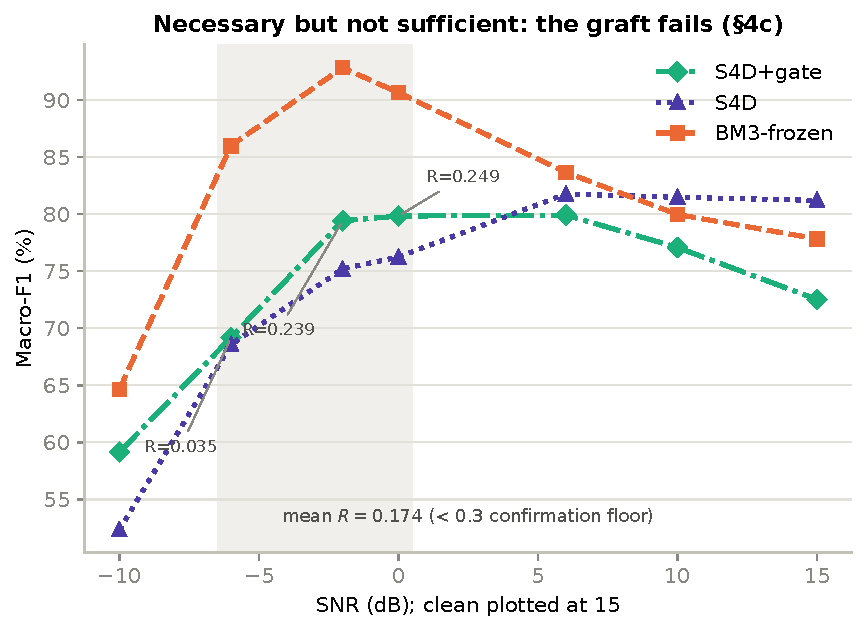
\includegraphics[width=0.85\linewidth]{figures/fig4_graft}
\caption{Graft outcome: S4D+gate, plain S4D, and BM3-frozen across the adjudication band, with the per-condition recovery ratio $R = (\text{S4D+gate} - \text{S4D})/(\text{frozen} - \text{S4D})$ annotated. Recovery is near zero at the deepest adjudicated noise level. This is the narrow graft; the width-matched graft and its additive control are in Table~\ref{tab:graftwm}.}
\label{fig:graft}
\end{figure}

Pre-specified recovery ratio $R = $ mean over the band of $(\text{S4D+gate} - \text{S4D})/(\text{frozen} - \text{S4D}) = \mathbf{0.174}$. The pre-specified bins were $R \geq 0.7$ (confirmed), $0.3 \leq R < 0.7$ (partial recovery) and $R < 0.3$ (insufficient); $R = 0.174$ falls in the last. Resampling seeds within each arm gives a 95\% interval of $[0.04, 0.29]$ for $R$, and the per-level paired gains of S4D+gate over S4D are $+3.6$ ($[-2.2, 9.3]$), $+4.2$ ($[1.1, 7.3]$) and $+0.6\pp$ ($[-2.2, 3.4]$). At the deepest adjudicated level the graft recovers essentially nothing. Removal and addition are not mirror-image interventions. In BM3 the gate has its own $64 \rightarrow 128$ projection and multiplies the scan output at the inner width of 128 before the output projection; removing it deletes $32{,}768$ parameters. In the S4D host the grafted gate is a $64 \rightarrow 64$ linear branch (with bias) computed from the layer input and multiplying the SSM output before the residual addition; it adds $16{,}640$ parameters over four layers. The two share the multiplicative SiLU form but not width, projection structure or parameter count. Removal costs $13$--$24\pp$ in the frozen block whereas this graft adds $0.6$--$4.2\pp$ to S4D. What this shows is that \emph{this gate branch, in this host and under this budget, recovers little}. Three readings fit the data and cannot be separated here: (i) host dependence, i.e.\ the gate needs the stem or scan context it co-trained with; (ii) implementation differences in width, projection and placement; (iii) transplant friction, i.e.\ the grafted branch is harder to optimise in a foreign host under the matched budget (training converges normally, but convergence is not robustness). Section~\ref{sec:results:graftwm} tests reading (ii) with a width-matched graft and an equal-capacity non-multiplicative control; a tuning or longer-budget comparison selected on a source-domain validation set was not run.

The four arms do allow a coarse host-by-gate contrast, $I = [F(\text{frozen}) - F(\text{frozen}{-}\text{gate})] - [F(\text{S4D+gate}) - F(\text{S4D})]$, where $F$ is macro-F1. Under last-epoch reporting $I = 5.2$ $[2.3, 8.1]$, $8.9$ $[-6.2, 23.9]$ and $22.6$ $[2.9, 42.4]\pp$ at $0$, $-2$ and $-6$\,dB (seed-matched 95\% $t$-intervals; positive in 5/5, 4/5 and 5/5 seeds); under best-epoch reporting in the re-run it is $7.8$ $[1.4, 14.2]$, $14.4$ $[-1.4, 30.3]$ and $23.1$ $[8.7, 37.4]\pp$. A positive $I$ means the gate adds more on the frozen host than on S4D. Because the host differs in several respects at once and the two gates are not aligned, $I$ cannot be assigned to a specific component or interaction term, and the seed pairing across arms is nominal (arms share seed indices, not initialisations).

\subsection{A width-matched graft and an additive control}
\label{sec:results:graftwm}

The graft of Section~\ref{sec:results:graft} is narrower and smaller than the donor gate. Two further arms rebuild it in the donor's shape (Table~\ref{tab:arms}). In each layer the layer input is projected to $x$ and $z$ of width 128 (the frozen block's inner width), the S4D layer runs on $x$ at width 128 with state size 64---so that its own parameter count and total state size equal the host's 64-wide, state-128 layer---and an output projection maps back to width 64. \emph{S4D+gate (wm)} combines $y \odot \mathrm{SiLU}(z)$, as the donor does; \emph{S4D+branch} uses the same modules, parameters and initial weights but combines $y + \mathrm{SiLU}(z)$. Both have 198{,}978 parameters, more than BM3-frozen (112{,}410) and BM3 (177{,}938), which biases the test towards recovery. A construction check with forward hooks confirms that the tensor entering the output projection equals the intended formula for each arm and not the other, and that the two arms are identical at initialisation. The thresholds were committed publicly before the grid ran (Section~\ref{sec:protocol:prereg}): $R$ as before, under final-epoch reporting; the verdict is INCONCLUSIVE whenever the seed-resampled interval crosses a bin boundary, in which case we write at the tier less favourable to the claim; and a gate-specific reading requires $\Delta R = R_{\text{gate}} - R_{\text{branch}} > 0.1$ with an interval excluding zero.

\begin{table}[htbp]
\centering
\caption{Width-matched graft and additive control on the original transition. Macro-F1 (\%), mean over 5 seeds, final-epoch reporting; $R$ is the mean over the three levels of (arm $-$ S4D)/(BM3-frozen $-$ S4D), with a seed-resampled 95\% interval. S4D, BM3-frozen and the narrow graft are the re-runs of Section~\ref{sec:results:sensitivity}.}
\label{tab:graftwm}
\footnotesize
\begin{tabular}{@{}lrrrcc@{}}
\toprule
Arm & 0\,dB & $-2$\,dB & $-6$\,dB & $R$ & 95\% interval \\
\midrule
S4D & 67.6 & 67.5 & 66.7 & -- & -- \\
S4D+gate (narrow) & 71.5 & 74.3 & 66.6 & 0.196 & [0.09, 0.31] \\
S4D+gate (wm) & 70.1 & 73.4 & 73.8 & 0.296 & [0.16, 0.52] \\
S4D+branch & 73.1 & 76.2 & 73.8 & 0.408 & [0.31, 0.60] \\
BM3-frozen & 83.1 & 87.3 & 83.1 & 1 & -- \\
\midrule
\multicolumn{4}{@{}l}{$\Delta R$ = S4D+gate (wm) $-$ S4D+branch} & $-0.112$ & [$-$0.26, 0.02] \\
\bottomrule
\end{tabular}
\end{table}

The width-matched graft recovers $R = 0.296$ of the gap (per level 0.159, 0.298, 0.431). Its interval, $[0.16, 0.52]$, crosses the 0.3 boundary, so the pre-specified verdict is INCONCLUSIVE between ``insufficient'' and ``partial'', and we report it at the less favourable tier: a graft built in the donor's shape recovers part of the gap. The recovery is not gate-specific. The additive branch, with the same parameters, recovers at least as much ($R = 0.408$), $\Delta R = -0.112$ $[-0.26, 0.02]$, and at 0\,dB the gated arm is below the additive one by $3.0\pp$ ($[-4.5, -1.5]$, 0/5 seeds). With frozen$-$all in the denominator the gated arm's ratio is $0.231$ $[0.13, 0.33]$; under best-epoch reporting the two ratios are 0.459 and 0.483. What a graft recovers on this transition therefore follows the added structure---a wider channel axis and input/output projections---rather than the multiplicative interaction. Reading (ii) of Section~\ref{sec:results:graft} is partly confirmed, in that the narrow graft understated what added structure can recover; but in the S4D host the gate itself contributes nothing beyond an equal-capacity additive branch, whereas removing it from the frozen Mamba-3 block costs $9$--$23\pp$ under the same rule (Table~\ref{tab:sensitivity_contrasts}).

\subsection{Replacing the gate in its native host}
\label{sec:results:nativeadd}

The previous subsection changes the host and keeps the operator. A pre-specified grid (15 cells, original transition) does the converse: it keeps the host and changes the operator. In \emph{frozen$+$add} the scan kernel of every BM3-frozen layer is called without gating and the layer output becomes $W_{\mathrm{out}}(y + \mathrm{SiLU}(z))$; modules, parameter count (112{,}410) and initial weights are bitwise those of BM3-frozen, and a construction check confirms that the donor operator is $y \odot \mathrm{SiLU}(z)$ and that the new arm computes $y + \mathrm{SiLU}(z)$. The pre-specified statistic is the native rescue ratio $\rho = (\text{add} - \text{no gate})/(\text{frozen} - \text{no gate})$, mean over levels, final epoch, with a seed-resampled interval; \emph{not rescued} requires $\rho < 0.3$ with an upper bound below $0.5$.

\begin{table}[htbp]
\centering
\caption{Gate replaced by an additive branch inside BM3-frozen (original transition). Macro-F1 (\%), mean over 5 seeds; paired differences under final-epoch reporting with 95\% $t$-intervals and the number of seeds (of 5) with a positive difference.}
\label{tab:nativeadd}
\footnotesize\setlength{\tabcolsep}{4pt}
\begin{tabular}{@{}lcccccc@{}}
\toprule
 & \multicolumn{2}{c}{0\,dB} & \multicolumn{2}{c}{$-2$\,dB} & \multicolumn{2}{c}{$-6$\,dB} \\
\cmidrule(lr){2-3}\cmidrule(lr){4-5}\cmidrule(lr){6-7}
Arm & best & final & best & final & best & final \\
\midrule
BM3-frozen ($y \odot \mathrm{SiLU}(z)$) & 90.6 & 83.1 & 92.3 & 87.3 & 85.7 & 83.1 \\
frozen$+$add ($y + \mathrm{SiLU}(z)$) & 78.0 & 74.7 & 72.6 & 71.5 & 62.3 & 60.9 \\
frozen$-$gate (no $z$) & 77.7 & 74.0 & 73.1 & 71.7 & 61.9 & 60.5 \\
\midrule
BM3-frozen $-$ frozen$+$add & \multicolumn{2}{c}{\shortstack{$+8.5$\\ {[}1.1, 15.9{]} (5/5)}} & \multicolumn{2}{c}{\shortstack{$+15.8$\\ {[}$-$1.2, 32.9{]} (4/5)}} & \multicolumn{2}{c}{\shortstack{$+22.2$\\ {[}4.6, 39.9{]} (5/5)}} \\[3pt]
frozen$+$add $-$ frozen$-$gate & \multicolumn{2}{c}{\shortstack{$+0.6$\\ {[}$-$1.7, 3.0{]} (3/5)}} & \multicolumn{2}{c}{\shortstack{$-0.2$\\ {[}$-$3.4, 3.0{]} (3/5)}} & \multicolumn{2}{c}{\shortstack{$+0.4$\\ {[}$-$0.7, 1.4{]} (3/5)}} \\[3pt]
\bottomrule
\end{tabular}
\end{table}

The additive branch rescues nothing. frozen$+$add is indistinguishable from the gateless arm at every level ($+0.6$, $-0.2$, $+0.4$\,pp, every interval including zero), and the multiplicative arm exceeds it by $8.5$, $15.8$, $22.2$\,pp. The rescue ratio is $\rho = 0.024$ (per level 0.070, $-$0.015, 0.016), with a seed-resampled 95\% interval of $[-1.159, 0.486]$; under best-epoch reporting $\rho = 0.005$. By the pre-specified rule the verdict is \emph{not rescued}. Two features of the interval should be read with it: its upper bound lies only $0.014$ below the threshold, and its lower bound is wide because the 0\,dB denominator is only $9.1\pp$ (in 7.8\% of resamples one level's denominator fell below $2\pp$ and was excluded, as pre-specified).

Together with Section~\ref{sec:results:graftwm} this gives the two halves of a symmetric test. In the S4D host the gate adds nothing beyond an additive branch of the same size; in the Mamba-3 host an additive branch of the same size adds nothing beyond removing the gate. The benefit of the gate is specific to the multiplicative operator \emph{in its native host}, and what transfers to the time-invariant host is the added structure, not the gating.

\subsection{The reverse transition}
\label{sec:results:reverse}

A pre-specified grid repeats the chain's central contrasts on the reverse transition, 40\,Hz/10\,kN $\rightarrow$ 37.5\,Hz/11\,kN (75 cells: frozen$-$all, BM3-frozen, frozen$-$gate, S4D and S4D+gate (wm), at three levels and five seeds; Section~\ref{sec:protocol:testbed} for the data). This direction is harder for the time-invariant model: on its evaluation set, predicting the majority class gives a macro-F1 of 46.8\% and uniform random guessing 41.5\%, and S4D sits close to those levels (Table~\ref{tab:reverse}).

\begin{table}[htbp]
\centering
\caption{Reverse transition (40\,Hz/10\,kN $\rightarrow$ 37.5\,Hz/11\,kN). Macro-F1 (\%), mean over 5 seeds, best-epoch and final-epoch reporting; paired differences under final-epoch reporting with 95\% $t$-intervals and the number of seeds (of 5) with a positive difference.}
\label{tab:reverse}
\footnotesize\setlength{\tabcolsep}{4pt}
\begin{tabular}{@{}lccc@{}}
\toprule
Arm (best / final) & 0\,dB & $-2$\,dB & $-6$\,dB \\
\midrule
frozen$-$all & 86.3 / 77.5 & 87.8 / 77.9 & 81.7 / 74.0 \\
BM3-frozen & 81.1 / 74.7 & 84.0 / 76.7 & 80.8 / 73.9 \\
S4D+gate (wm) & 79.0 / 72.9 & 80.5 / 73.9 & 78.5 / 72.2 \\
frozen$-$gate & 63.8 / 56.2 & 62.0 / 54.7 & 57.1 / 50.0 \\
S4D & 61.2 / 51.2 & 61.0 / 52.4 & 54.6 / 51.8 \\
\midrule
frozen$-$all $-$ S4D & \shortstack{$+26.3$\\ {[}21.5, 31.0{]} (5/5)} & \shortstack{$+25.6$\\ {[}21.1, 30.1{]} (5/5)} & \shortstack{$+22.2$\\ {[}18.8, 25.6{]} (5/5)} \\[3pt]
BM3-frozen $-$ frozen$-$gate & \shortstack{$+18.4$\\ {[}1.2, 35.6{]} (5/5)} & \shortstack{$+22.0$\\ {[}3.4, 40.6{]} (5/5)} & \shortstack{$+24.0$\\ {[}7.6, 40.3{]} (5/5)} \\[3pt]
frozen$-$gate $-$ S4D & \shortstack{$+5.0$\\ {[}$-$17.6, 27.7{]} (2/5)} & \shortstack{$+2.4$\\ {[}$-$19.2, 23.9{]} (2/5)} & \shortstack{$-1.8$\\ {[}$-$18.9, 15.3{]} (1/5)} \\[3pt]
S4D+gate (wm) $-$ S4D & \shortstack{$+21.7$\\ {[}15.4, 28.0{]} (5/5)} & \shortstack{$+21.5$\\ {[}17.0, 26.0{]} (5/5)} & \shortstack{$+20.5$\\ {[}15.7, 25.2{]} (5/5)} \\[3pt]
\bottomrule
\end{tabular}
\end{table}

The first two steps replicate. The fully input-independent scan exceeds S4D by $+26.3$, $+25.6$ and $+22.2\pp$ at $0$, $-2$ and $-6$\,dB, with intervals excluding zero and 5/5 seeds at every level, so by the pre-specified rule (at least two of three levels) the first step is replicated on the reverse transition. Removing the gate from BM3-frozen costs $18.4$, $22.0$ and $24.0\pp$, above the $8\pp$ threshold at all three levels, with intervals excluding zero and 5/5 seeds, and the gateless arm is indistinguishable from S4D (intervals include zero). On the third step, which the pre-specification treats as descriptive here, the width-matched graft recovers most of the gap, $R = 0.911$ $[0.82, 1.04]$ ($0.863$ with frozen$-$all in the denominator). A further pre-specified grid (15 cells) adds the same-size additive control in this direction: it reaches 67.8, 72.1, 68.4\% (final epoch) and recovers $R = 0.758$ $[0.66, 0.88]$. The gate arm exceeds it by $+5.1$, $+1.7$, $+3.8$\,pp (only the $-6$\,dB interval excludes zero), and the difference in recovery is $\Delta R = 0.153$ $[0.06, 0.26]$; under best-epoch reporting it shrinks to $0.037$ $[-0.1, 0.17]$. By the pre-specified descriptive labels this is \emph{unresolved}: in this direction the gate carries a small increment over the additive branch, whereas on the original transition it carried none ($\Delta R = -0.112$). Most of the reverse-direction recovery is therefore available to an additive branch of the same size, and the remaining gate increment is direction-dependent. Both ratios rest on an S4D baseline close to the trivial floor (51--52\% against 46.8\% for the majority class). Both statements carry the limits of this pair: the same eight bearings with their roles swapped, and a single inner-race bearing in the evaluation set.

\subsection{Sensitivity to the reporting rule}
\label{sec:results:sensitivity}

The tables above use best-epoch macro-F1 on the evaluation condition (Section~\ref{sec:protocol:report}). To measure how much this rule shapes the conclusions, we re-ran the four arms that carry the chain (BM3-frozen, S4D, frozen$-$gate, S4D+gate) over the adjudication band: 60 cells, 5 seeds, 50 epochs, the original training code and the same evaluation fingerprint, recording macro-F1 at every epoch and reporting it at the final epoch, where the cosine learning-rate schedule has annealed to zero. This rule uses no evaluation data to pick a model. The re-run used a different PyTorch/Triton build from the original grids; its best-epoch values reproduce the original arm-by-condition means to within $-0.6$ to $+1.4\pp$ (the largest deviation is in the high-variance frozen$-$gate arm at $-2$\,dB). The S4D-wide capacity control and the conv-stem and $A$-parameterisation ablations were not re-run; the original BM3 arm was re-run in the stage-2 grid of Section~\ref{sec:results:fullfreeze}, so $\Delta$(BM3$-$frozen) is available under both rules.

\begin{table}[htbp]
\centering
\caption{Macro-F1 (\%), mean over 5 seeds, under best-epoch reporting (re-run) and final-epoch reporting.}
\label{tab:sensitivity_means}
\begin{tabular}{@{}lrrrrrr@{}}
\toprule
 & \multicolumn{2}{c}{0\,dB} & \multicolumn{2}{c}{$-2$\,dB} & \multicolumn{2}{c}{$-6$\,dB} \\
\cmidrule(lr){2-3}\cmidrule(lr){4-5}\cmidrule(lr){6-7}
Arm & best & final & best & final & best & final \\
\midrule
BM3-frozen & 90.6 & 83.1 & 92.3 & 87.3 & 85.7 & 83.1 \\
S4D & 75.9 & 67.6 & 75.1 & 67.5 & 68.6 & 66.7 \\
frozen$-$gate & 77.7 & 74.0 & 73.1 & 71.7 & 61.9 & 60.5 \\
S4D+gate & 80.9 & 71.5 & 79.9 & 74.3 & 69.2 & 66.6 \\
\bottomrule
\end{tabular}
\end{table}

Final-epoch values are lower than best-epoch values by $1.4$--$9.5\pp$ across the twelve arm-by-level means, so the absolute levels in Tables~\ref{tab:falsify}--\ref{tab:graft} are optimistic. The reduction is of similar size for the arms being contrasted (e.g., BM3-frozen $-7.4$, $-5.0$, $-2.6\pp$ and S4D $-8.3$, $-7.6$, $-1.9\pp$ at $0$, $-2$, $-6$\,dB), and the contrasts that carry the argument are correspondingly stable (Table~\ref{tab:sensitivity_contrasts}).

\begin{table}[htbp]
\centering
\caption{Paired differences under final-epoch reporting, in percentage points: mean, 95\% $t$-interval over seeds, and number of seeds (of 5) with a positive difference.}
\label{tab:sensitivity_contrasts}
\footnotesize\setlength{\tabcolsep}{4pt}
\begin{tabular}{@{}lccc@{}}
\toprule
Contrast & 0\,dB & $-2$\,dB & $-6$\,dB \\
\midrule
BM3-frozen $-$ S4D & \shortstack{$+15.5$\\ {[}4.3, 26.8{]} (5/5)} & \shortstack{$+19.8$\\ {[}12.0, 27.7{]} (5/5)} & \shortstack{$+16.4$\\ {[}4.1, 28.7{]} (4/5)} \\[3pt]
BM3-frozen $-$ frozen$-$gate & \shortstack{$+9.1$\\ {[}2.9, 15.3{]} (5/5)} & \shortstack{$+15.6$\\ {[}$-$0.8, 32.0{]} (4/5)} & \shortstack{$+22.6$\\ {[}5.8, 39.4{]} (5/5)} \\[3pt]
frozen$-$gate $-$ S4D & \shortstack{$+6.4$\\ {[}$-$2.9, 15.8{]} (4/5)} & \shortstack{$+4.2$\\ {[}$-$14.5, 22.9{]} (3/5)} & \shortstack{$-6.2$\\ {[}$-$23.5, 11.2{]} (1/5)} \\[3pt]
S4D+gate $-$ S4D & \shortstack{$+3.9$\\ {[}$-$0.8, 8.6{]} (4/5)} & \shortstack{$+6.8$\\ {[}2.4, 11.1{]} (5/5)} & \shortstack{$-0.1$\\ {[}$-$4.0, 3.9{]} (2/5)} \\[3pt]
\bottomrule
\end{tabular}
\end{table}

\emph{Selectivity.} The frozen block's advantage over S4D is $+15.5$, $+19.8$ and $+16.4\pp$ (and $+21.9$, $+24.0$, $+21.2\pp$ for the fully frozen scan, Section~\ref{sec:results:fullfreeze}), versus $+14.6$, $+17.2$ and $+17.1\pp$ under best-epoch reporting in the re-run. It remains positive in 5/5, 5/5 and 4/5 seeds, with intervals excluding zero at every level. \emph{Gate.} Removing the gate costs $9.1$, $15.6$ and $22.6\pp$ ($12.8$ to $23.8\pp$ under best-epoch reporting in the re-run), above the $8\pp$ pre-specified threshold at every level; the interval at $-2$\,dB includes zero ($[-0.8, 32.0]\pp$, 4/5 seeds) because of the large seed variance of the gateless arm (standard deviation $14.6\pp$ at $-2$\,dB). \emph{Gateless versus S4D.} Under final-epoch reporting the gateless arm is not below S4D at $0$ and $-2$\,dB (point estimates $+6.4$ and $+4.2\pp$) and is below it at $-6$\,dB ($-6.2\pp$); all three intervals include zero. The statement that gate removal ``falls below S4D'' is therefore supported only as a point-estimate observation at the deepest level, and we phrase it as ``to or below'' elsewhere. \emph{Graft.} The recovery ratio is $0.249$, $0.341$ and $-0.003$ per level and $R = 0.196$ on average (best-epoch re-run: $0.220$), again in the pre-specified ``insufficient'' bin on the point estimate. The seed-resampled 95\% interval is $[0.09, 0.31]$ and so reaches the $0.3$ boundary: with five seeds the data support ``far below confirmation ($0.7$) and probably below $0.3$'', not a precise value of $R$. The graft gain over S4D is resolved at $-2$\,dB only ($+6.8\pp$, $[2.4, 11.1]$) and is indistinguishable from zero at $-6$\,dB.

Because the final epoch of the same evaluation condition has been inspected repeatedly during this study, last-epoch values are also not a fresh confirmatory test. The reporting rule therefore changes absolute levels and the strength of the gateless-versus-S4D statement, but not the ordering BM3-frozen $>$ \{S4D+gate, frozen$-$gate, S4D\}, the size of the frozen block's advantage over S4D, or the verdicts of the pre-specified gate and graft rules.

\subsection{The interaction effect concentrates on the hard class}
\label{sec:results:perclass}

\begin{figure}[htbp]
\centering
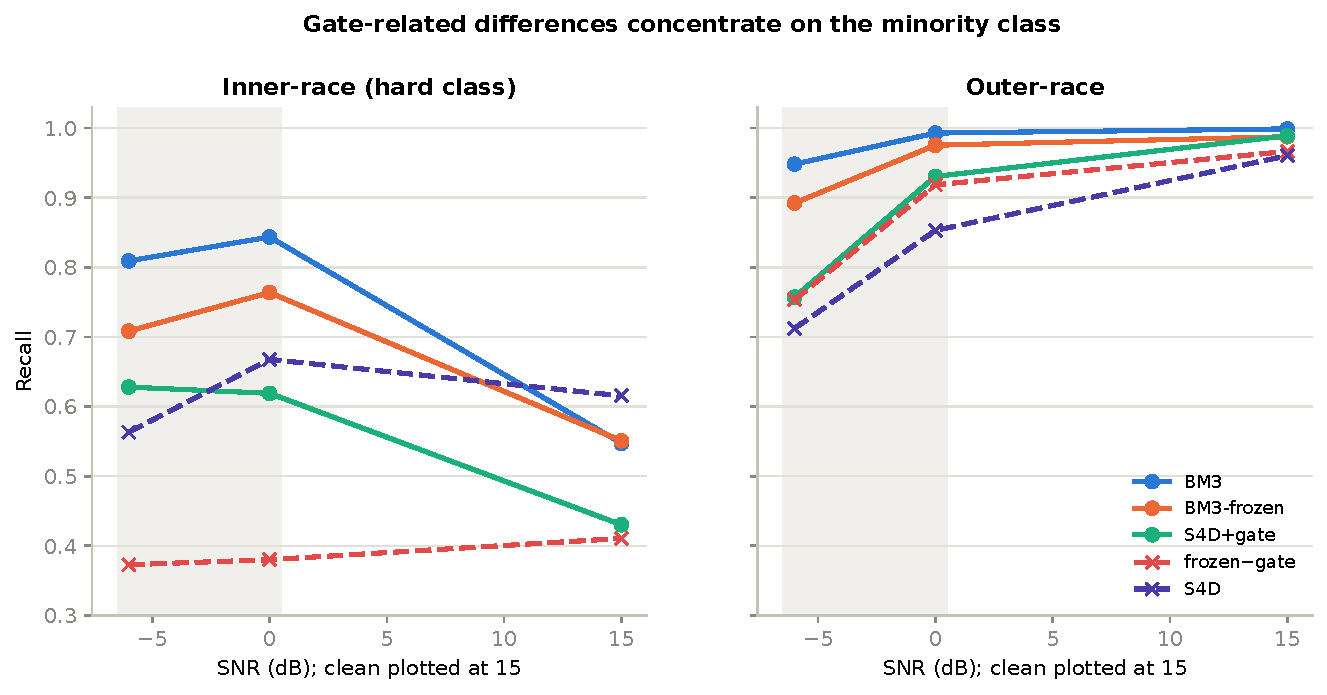
\includegraphics[width=0.85\linewidth]{figures/fig5_perclass}
\caption{Per-class recall (inner-race, IR, and outer-race, OR) as a function of noise depth, split by gate presence. Gated arms lift IR recall under matched noise; gateless arms let it deteriorate.}
\label{fig:perclass}
\end{figure}

Per-class analysis (a separate 75-cell grid at 20 epochs with best-epoch selection on the evaluation condition: 5 arms $\times$ $\{$clean, 0, $-6\,\mathrm{dB}\}$ $\times$ 5 seeds, per-sample predictions dumped and re-verified against reported metrics cell-by-cell): the inner-race class is hard from the outset (clean recall $0.41$--$0.62$ vs.\ $0.96$--$1.00$ for outer-race). Its trajectory under noise is governed by gate presence: in all three gated arms IR recall at $-6$\,dB exceeds its clean value (e.g., $0.55 \rightarrow 0.81$ for BM3), while in both gateless arms it is below its clean value (frozen$-$gate: $0.41 \rightarrow 0.37$; S4D: $0.62 \rightarrow 0.56$, non-monotone, rising to $0.67$ at $0$\,dB) (Figure~\ref{fig:perclass}). Both ablation directions hit IR hardest---gate removal costs IR $2.3$--$3.8\times$ more F1 than OR at every level (F1 from predictions pooled over seeds), and the graft's noise-time gains also concentrate on IR ($-6$\,dB: $+6.8\pp$ IR vs.\ $+4.2\pp$ OR). Because macro-F1 averages the two classes, the arm-level robustness gaps of Sections~\ref{sec:results:falsify}--\ref{sec:results:graft} are carried substantially by the hard class. The gate-related differences are therefore class-concentrated rather than uniform, and fall on the class with the lowest recall. We did not measure classification margins, so we do not describe IR as a ``low-margin'' class. Because this grid is separate from the main 50-epoch grid and the IR class comes from a single training bearing (Section~\ref{sec:protocol:testbed}), these results are descriptive and do not decompose the main-grid effects.
